\documentclass[9pt, notheorems]{beamer}
\setcounter{tocdepth}{4}
\usepackage[utf8]{inputenc}
\usepackage[T1]{fontenc}
\usepackage{lmodern}
\usepackage{amsmath}
\usepackage{mathdots}
\usepackage{amsthm}
\usepackage{amssymb}
\usepackage{mathrsfs}
\usepackage{amsfonts}
\usepackage{stmaryrd}
\usepackage{xfrac}
\usepackage{dsfont}
\usepackage{fancybox}
\usepackage{fancyref}
\usepackage{multicol}
\usepackage{graphicx}
\usepackage{wrapfig}
\usepackage{textcomp}
\usepackage{mathrsfs}
\usepackage{color}
\usepackage{listings}
\usepackage{tikz-cd}
\usepackage{comment}
\usepackage{caption}
\usepackage{shuffle}
\usepackage{multirow}
\usepackage{appendix}
\usepackage{fdsymbol}
\usepackage{float}
\usepackage{algorithm}
\usepackage[noend]{algpseudocode}
\usepackage{qcircuit}
\usepackage{hyperref}

\newcommand{\HRule}{\rule{\linewidth}{0.5mm}}
\newcommand{\Dyck}[1]{\textsc{Dyck$_{#1}$}}
\newcommand{\FA}[1]{\textsc{FindAny$_{#1}$}}
\newcommand{\FFL}[1]{\textsc{FindFixedLength$_{#1}$}}
\newcommand{\FFP}[1]{\textsc{FindFixedPos$_{#1}$}}
\newcommand{\FALM}[1]{\textsc{FindAtLeftMost$_{#1}$}}
\newcommand{\FARM}[1]{\textsc{FindAtRightMost$_{#1}$}}
\newcommand{\FF}[1]{\textsc{FindFirst$_{#1}$}}
\newcommand{\Null}{\textsc{Null}}

\newcommand{\hered}[1]{\paragraph*{Induction:}{#1}}
\newcommand{\init}[1]{\paragraph*{Initialization:}{#1}}
\newcommand{\IH}[1]{\paragraph*{Induction Hypothesis:}{#1}}
\newcommand{\Conc}[1]{\paragraph*{Conclusion:}{#1}}
\newcommand{\remark}[1]{\paragraph*{Remark:}{#1}}
\newcommand{\observation}[1]{\paragraph*{Observation:}{#1}}
\newcommand{\notation}[1]{\paragraph*{Notation:}{#1}}
\newcommand{\property}[1]{\paragraph*{Property:}{#1}}
\newcommand{\ket}[1]{\ensuremath{|#1\rangle}}
\newcommand{\metersymbol}[1]{\begin{tikzpicture}[scale=#1]
    \draw (.8, 0) arc (0:180:.8);
    \draw[->] (0, 0) -- (1, 1);
\end{tikzpicture}
    }

\renewcommand{\comment}[1]{}
\newcommand\blfootnote[1]{%
    \begingroup
    \renewcommand\thefootnote{}\footnote{#1}%
    \addtocounter{footnote}{-1}%
    \endgroup
}

\newlength\myindent
\setlength\myindent{2em}
\newcommand\bindent{%
  \begingroup
  \setlength{\itemindent}{\myindent}
  \addtolength{\algorithmicindent}{\myindent}
}
\newcommand\eindent{\endgroup}

\theoremstyle{definition}
\newtheorem{definition}{Définition}
\newtheorem{proposition}{Proposition}[definition]

\theoremstyle{plain}
\newtheorem{theorem}{Theorem}[section]
\newtheorem{corollary}{Corollary}[theorem]
\newtheorem{lemma}{Lemma}[theorem]

\theoremstyle{definition}
\newtheorem{conjecture}{Conjecture}[definition]
\newtheorem{cproof}{Proof Corollary}[theorem] 
\newtheorem{lproof}{Proof Lemma}[theorem]
\newtheorem{tproof}{Proof Theorem}[section]

\usetheme{Warsaw}
\usefonttheme{professionalfonts}

\title[QQC of bounded height Dyck languages.]{{\huge Complexity of recognizing Dyck languages
of bounded height with quantum query algorithms.}}
\author{Maxime CAUTRÈS}
\institute{Faculty of Computing\\ University of Latvia}
\date{31/08/2022}

\addtobeamertemplate{footline}{\ \insertframenumber/\inserttotalframenumber\ }

\AtBeginSection[]
{
  \begin{frame}
  \frametitle{Sommaire}
  \tableofcontents[currentsection, hideothersubsections]
  \end{frame} 
}

\begin{document}

\begin{frame}
    \titlepage
\end{frame}

\section{Introduction}

\comment{}
\subsection{Quantum query model and complexity}

\comment{
\begin{frame}
    \frametitle{Classical and quantum computers are both made with simple components.}
    \begin{minipage}{.45\textwidth}
        \begin{figure}
            \tikzset{every picture/.style={line width=0.75pt}} %set default line width to 0.75pt        
\centering
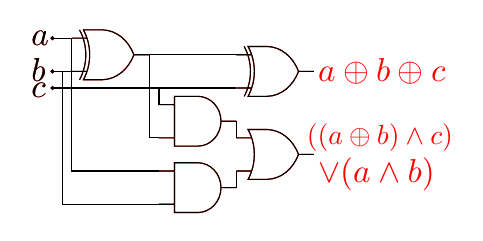
\begin{tikzpicture}[x=0.70pt,y=0.60pt,yscale=-.5,xscale=.5]
    %uncomment if require: \path (0,300); %set diagram left start at 0, and has height of 300

    \visible<1>{
        % Text Node
        \draw[red] (15,48) node [anchor=north west][inner sep=0.75pt]  [xscale=1.2,yscale=1.2] [align=left] {$a$};
        % Text Node
        \draw[red] (15,80) node [anchor=north west][inner sep=0.75pt]  [xscale=1.2,yscale=1.2] [align=left] {$b$};
        % Text Node
        \draw[red] (15,110) node [anchor=north west][inner sep=0.75pt]  [xscale=1.2,yscale=1.2] [align=left] {$c$};

        \filldraw[red] (40, 60) circle (1pt);
        \filldraw[red] (40, 100) circle (1pt);
        \filldraw[red] (40, 120) circle (1pt);
    }
    \visible<2->{
        % Text Node
        \draw (15,48) node [anchor=north west][inner sep=0.75pt]  [xscale=1.2,yscale=1.2] [align=left] {$a$};
        % Text Node
        \draw (15,80) node [anchor=north west][inner sep=0.75pt]  [xscale=1.2,yscale=1.2] [align=left] {$b$};
        % Text Node
        \draw (15,110) node [anchor=north west][inner sep=0.75pt]  [xscale=1.2,yscale=1.2] [align=left] {$c$};

        \filldraw (40, 60) circle (1pt);
        \filldraw (40, 100) circle (1pt);
        \filldraw (40, 120) circle (1pt);
    }

    \visible<2>{
        %Shape: Xor Gate [id:dp7586863585025112] 
        \draw[red]   (72,50) -- (92,50) .. controls (105.95,50.54) and (118.42,62.23) .. (124,80) .. controls (118.42,97.77) and (105.95,109.46) .. (92,110) -- (72,110) .. controls (80.57,91.44) and (80.57,68.56) .. (72,50) -- cycle (60,60) -- (76,60) (60,100) -- (76,100) (124,80) -- (140,80) (68,50) .. controls (76.57,68.56) and (76.57,91.44) .. (68,110) ;
        %Shape: Xor Gate [id:dp4857055310285392] 
        \draw[red]   (242,70) -- (262,70) .. controls (275.95,70.54) and (288.42,82.23) .. (294,100) .. controls (288.42,117.77) and (275.95,129.46) .. (262,130) -- (242,130) .. controls (250.57,111.44) and (250.57,88.56) .. (242,70) -- cycle (230,80) -- (246,80) (230,120) -- (246,120) (294,100) -- (310,100) (238,70) .. controls (246.57,88.56) and (246.57,111.44) .. (238,130) ;
        %Shape: And Gate [id:dp40243073644089766] 
        \draw[red]   (166,130) -- (190,130) .. controls (203.25,130) and (214,143.44) .. (214,160) .. controls (214,176.56) and (203.25,190) .. (190,190) -- (166,190) -- (166,130) -- cycle (150,140) -- (166,140) (150,180) -- (166,180) (214,160) -- (230,160) ;
        %Shape: And Gate [id:dp08349658070673471] 
        \draw[red]   (166,210) -- (190,210) .. controls (203.25,210) and (214,223.44) .. (214,240) .. controls (214,256.56) and (203.25,270) .. (190,270) -- (166,270) -- (166,210) -- cycle (150,220) -- (166,220) (150,260) -- (166,260) (214,240) -- (230,240) ;
        %Shape: Or Gate [id:dp5052546687696813] 
        \draw[red]   (242,170) -- (262,170) .. controls (275.95,170.54) and (288.42,182.23) .. (294,200) .. controls (288.42,217.77) and (275.95,229.46) .. (262,230) -- (242,230) .. controls (250.57,211.44) and (250.57,188.56) .. (242,170) -- cycle (230,180) -- (246,180) (230,220) -- (246,220) (294,200) -- (310,200) ;
    }
    \visible<3->{
        %Shape: Xor Gate [id:dp7586863585025112] 
        \draw   (72,50) -- (92,50) .. controls (105.95,50.54) and (118.42,62.23) .. (124,80) .. controls (118.42,97.77) and (105.95,109.46) .. (92,110) -- (72,110) .. controls (80.57,91.44) and (80.57,68.56) .. (72,50) -- cycle (60,60) -- (76,60) (60,100) -- (76,100) (124,80) -- (140,80) (68,50) .. controls (76.57,68.56) and (76.57,91.44) .. (68,110) ;
        %Shape: Xor Gate [id:dp4857055310285392] 
        \draw   (242,70) -- (262,70) .. controls (275.95,70.54) and (288.42,82.23) .. (294,100) .. controls (288.42,117.77) and (275.95,129.46) .. (262,130) -- (242,130) .. controls (250.57,111.44) and (250.57,88.56) .. (242,70) -- cycle (230,80) -- (246,80) (230,120) -- (246,120) (294,100) -- (310,100) (238,70) .. controls (246.57,88.56) and (246.57,111.44) .. (238,130) ;
        %Shape: And Gate [id:dp40243073644089766] 
        \draw   (166,130) -- (190,130) .. controls (203.25,130) and (214,143.44) .. (214,160) .. controls (214,176.56) and (203.25,190) .. (190,190) -- (166,190) -- (166,130) -- cycle (150,140) -- (166,140) (150,180) -- (166,180) (214,160) -- (230,160) ;
        %Shape: And Gate [id:dp08349658070673471] 
        \draw   (166,210) -- (190,210) .. controls (203.25,210) and (214,223.44) .. (214,240) .. controls (214,256.56) and (203.25,270) .. (190,270) -- (166,270) -- (166,210) -- cycle (150,220) -- (166,220) (150,260) -- (166,260) (214,240) -- (230,240) ;
        %Shape: Or Gate [id:dp5052546687696813] 
        \draw   (242,170) -- (262,170) .. controls (275.95,170.54) and (288.42,182.23) .. (294,200) .. controls (288.42,217.77) and (275.95,229.46) .. (262,230) -- (242,230) .. controls (250.57,211.44) and (250.57,188.56) .. (242,170) -- cycle (230,180) -- (246,180) (230,220) -- (246,220) (294,200) -- (310,200) ;
    }
    \visible<3>{
        %Straight Lines [id:da47322578625017586] 
        \draw[red]    (40,60) -- (60,60) ;
        %Straight Lines [id:da9794654949941013] 
        \draw[red]    (230,160) -- (230,180) ;
        %Straight Lines [id:da4846849793546657] 
        \draw[red]    (230,220) -- (230,240) ;
        %Straight Lines [id:da5854134933106738] 
        \draw[red]    (140,80) -- (140,120) -- (140,180) ;
        %Straight Lines [id:da21543002534508293] 
        \draw[red]    (150,180) -- (140,180) ;
        %Straight Lines [id:da2647954495406195] 
        \draw[red]    (40,120) -- (140.33,120) -- (230,120) ;
        %Straight Lines [id:da3173932178858232] 
        \draw[red]    (40,100) -- (60,100) ;
        %Straight Lines [id:da4191196124425738] 
        \draw[red]    (150,120) -- (150,140) ;
        %Straight Lines [id:da7200697769419422] 
        \draw[red]    (60,60) -- (60,220) -- (150,220) ;
        %Straight Lines [id:da6864505677890691] 
        \draw[red]    (50,100) -- (50,260) -- (150,260) ;
        %Straight Lines [id:da27064207791990746] 
        \draw[red]    (139.67,80) -- (140,80) -- (239.67,80) ;}
    \visible<4->{
        %Straight Lines [id:da47322578625017586] 
        \draw    (40,60) -- (60,60) ;
        %Straight Lines [id:da9794654949941013] 
        \draw    (230,160) -- (230,180) ;
        %Straight Lines [id:da4846849793546657] 
        \draw    (230,220) -- (230,240) ;
        %Straight Lines [id:da5854134933106738] 
        \draw    (140,80) -- (140,120) -- (140,180) ;
        %Straight Lines [id:da21543002534508293] 
        \draw    (150,180) -- (140,180) ;
        %Straight Lines [id:da2647954495406195] 
        \draw    (40,120) -- (140.33,120) -- (230,120) ;
        %Straight Lines [id:da3173932178858232] 
        \draw    (40,100) -- (60,100) ;
        %Straight Lines [id:da4191196124425738] 
        \draw    (150,120) -- (150,140) ;
        %Straight Lines [id:da7200697769419422] 
        \draw    (60,60) -- (60,220) -- (150,220) ;
        %Straight Lines [id:da6864505677890691] 
        \draw    (50,100) -- (50,260) -- (150,260) ;
        %Straight Lines [id:da27064207791990746] 
        \draw    (139.67,80) -- (140,80) -- (239.67,80) ;}

    \visible<4->{
        % Text Node
        \draw[red] (311,80) node [anchor=north west][inner sep=0.75pt]  [xscale=1.2,yscale=1.2] [align=left] {$a\oplus b\oplus c$};
        % Text Node
        \draw[red] (300,160) node [anchor=north west][inner sep=0.75pt]  [xscale=1,yscale=1] [align=left] {$(( a\oplus b) \land c)$};
        % Text Node
        \draw[red] (311,200) node [anchor=north west][inner sep=0.75pt]  [xscale=1.2,yscale=1.2] [align=left] {$ \lor ( a\land b)$};
    }


\end{tikzpicture}
            \caption{A Boolean circuit (Full adder).}
        \end{figure}
    \end{minipage}
    \hfill
    \begin{minipage}{.45\textwidth}
        \begin{figure}
            \vspace*{.5cm}
            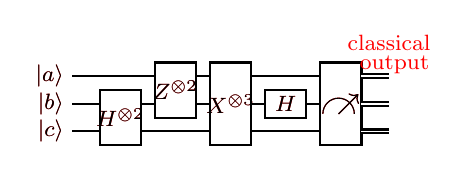
\begin{tikzpicture}[scale=.35]
    \footnotesize
    \visible<1>{
        \draw[red] (-1, 2.5) node[left] {$\ket{a}$};
        \draw[red] (-1, 1.5) node[left] {$\ket{b}$};
        \draw[red] (-1, .5) node[left] {$\ket{c}$};}

    \visible<2->{
        \draw (-1, 2.5) node[left] {$\ket{a}$};
        \draw (-1, 1.5) node[left] {$\ket{b}$};
        \draw (-1, .5) node[left] {$\ket{c}$};}


    \visible<2>{
        \draw[red, thick] (0,0) -- (1.5, 0) -- (1.5, 2) -- (0, 2) -- cycle;
        \draw[thick, red] (2+0,0+1) -- (2+1.5, 0+1) -- (2+1.5, 2+1) -- (2+0, 2+1) -- cycle;
        \draw[thick,red] (4+0,0) -- (4+1.5, 0) -- (4+1.5, 3) -- (4+0, 3) -- cycle;
        \draw[thick,red] (6,0+1) -- (6, 2) -- (7.5, 2) -- (7.5, 1) -- cycle;
        \draw[thick,red] (8+0,0) -- (8+1.5, 0) -- (8+1.5, 3) -- (8+0, 3) -- cycle;
        \draw[red] (.75, 1) node {$H^{\otimes2}$};
        \draw[red] (2.75, 2) node {$Z^{\otimes2}$};
        \draw[red] (4.75, 1.5) node {$X^{\otimes3}$};
        \draw[red] (6.75, 1.5) node {$H$};
        \draw[red] (8.75, 1.5) node {$\metersymbol{.25}$};}

    \visible<3->{
        \draw[thick] (0,0) -- (1.5, 0) -- (1.5, 2) -- (0, 2) -- cycle;
        \draw[thick] (2+0,0+1) -- (2+1.5, 0+1) -- (2+1.5, 2+1) -- (2+0, 2+1) -- cycle;
        \draw[thick] (4+0,0) -- (4+1.5, 0) -- (4+1.5, 3) -- (4+0, 3) -- cycle;
        \draw[thick] (6,0+1) -- (6, 2) -- (7.5, 2) -- (7.5, 1) -- cycle;
        \draw[thick] (8+0,0) -- (8+1.5, 0) -- (8+1.5, 3) -- (8+0, 3) -- cycle;
        \draw (.75, 1) node {$H^{\otimes2}$};
        \draw (2.75, 2) node {$Z^{\otimes2}$};
        \draw (4.75, 1.5) node {$X^{\otimes3}$};
        \draw (6.75, 1.5) node {$H$};
        \draw (8.75, 1.5) node {$\metersymbol{.25}$};}

    \visible<3>{

        \draw[red,thick] (-1, .5) -- (0, .5);
        \draw[red,thick] (1.5, .5) -- (4, .5);
        \draw[red,thick] (5.5, .5) -- (8, .5);
        \draw[red,thick, double] (9.5, .5) -- (10.5, 0.5);


        \draw[red,thick] (-1, 1.5) -- (0, 1.5);
        \draw[red,thick] (1.5, 1.5) -- (2, 1.5);
        \draw[red,thick] (3.5, 1.5) -- (4, 1.5);
        \draw[red,thick] (5.5, 1.5) -- (6, 1.5);
        \draw[red,thick] (7.5, 1.5) -- (8, 1.5);
        \draw[red,thick, double] (9.5, 1.5) -- (10.5, 1.5);


        \draw[red,thick] (-1, 2.5) -- (2, 2.5);
        \draw[red,thick] (3.5, 2.5) -- (4, 2.5);
        \draw[red,thick] (5.5, 2.5) -- (8, 2.5);
        \draw[red,thick, double] (9.5, 2.5) -- (10.5, 2.5);}

    \visible<4->{

        \draw[thick] (-1, .5) -- (0, .5);
        \draw[thick] (1.5, .5) -- (4, .5);
        \draw[thick] (5.5, .5) -- (8, .5);
        \draw[thick, double] (9.5, .5) -- (10.5, 0.5);


        \draw[thick] (-1, 1.5) -- (0, 1.5);
        \draw[thick] (1.5, 1.5) -- (2, 1.5);
        \draw[thick] (3.5, 1.5) -- (4, 1.5);
        \draw[thick] (5.5, 1.5) -- (6, 1.5);
        \draw[thick] (7.5, 1.5) -- (8, 1.5);
        \draw[thick, double] (9.5, 1.5) -- (10.5, 1.5);


        \draw[thick] (-1, 2.5) -- (2, 2.5);
        \draw[thick] (3.5, 2.5) -- (4, 2.5);
        \draw[thick] (5.5, 2.5) -- (8, 2.5);
        \draw[thick, double] (9.5, 2.5) -- (10.5, 2.5);}

    \visible<4>{
        \draw[red] (10.5, 3.7) node {classical};
        \draw[red] (10.7, 2.9) node {output};}

\end{tikzpicture}\\[.8cm]
            \caption{A Quantum circuit.}
        \end{figure}
    \end{minipage}
\end{frame}}

\begin{frame}
    \frametitle{Interacting with qubits is more complexe.}

    \begin{minipage}{.45\textwidth}
        \visible<1->{
            \begin{figure}
                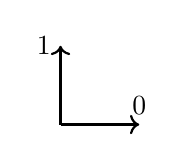
\begin{tikzpicture}
                    \draw[thick, ->] (0, 0) -- (1, 0);
                    \draw[thick, ->] (0, 0) -- (0, 1);
                    \draw (1, 0) node[above] {0};
                    \draw (0, 1) node[left] {1};
                \end{tikzpicture}
                \caption{A classical bit}
            \end{figure}}
        \visible<3->{
            \begin{figure}
                \begin{tabular}{c|c||c}
                    $A$ & $B$ & $A\oplus B$ \\
                    \hline
                    0   & 0   & 0           \\
                    0   & 1   & 1           \\
                    1   & 0   & 1           \\
                    1   & 1   & 0           \\
                \end{tabular}
                \caption{Truth table on 2 bits.}
            \end{figure}}
    \end{minipage}
    \hfill
    \begin{minipage}{.45\textwidth}
        \visible<2->{
            \begin{figure}
                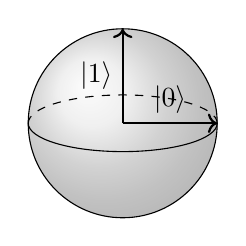
\begin{tikzpicture}[scale=.6]
                    \shade[ball color = gray!40, opacity = 0.4] (0,0) circle (2cm);
                    \draw (0,0) circle (2cm);
                    \draw (-2,0) arc (180:360:2 and 0.6);
                    \draw[dashed] (2,0) arc (0:180:2 and 0.6);
                    \draw[thick, ->] (0,0 ) -- node[above]{$\ket{0}$} (2,0);
                    \draw[thick, ->] (0,0) -- node[left]{$\ket{1}$} (0, 2);
                \end{tikzpicture}
                \caption{A quantum bit.}
            \end{figure}}
        \visible<4->{
            \begin{figure}
                $H^{\otimes2} =\frac{1}{2}
                    \begin{bmatrix}
                        1 & 1  & 1  & 1  \\
                        1 & -1 & 1  & -1 \\
                        1 & 1  & -1 & -1 \\
                        1 & -1 & -1 & 1
                    \end{bmatrix}$
                \caption{Unitary matrix on 2 qubits.}
            \end{figure}}
    \end{minipage}
\end{frame}

\begin{frame}
    \frametitle{Quantum query algorithm is just a quantum circuit.}
    \visible<1->{{
                \huge \[x = \underbrace{100101\ldots01011}_{n}\]}}
    \begin{figure}
        \centering

        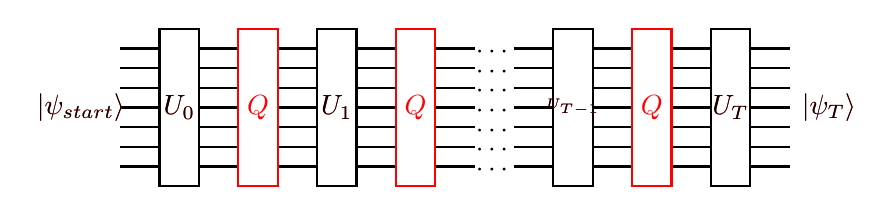
\begin{tikzpicture}[scale=.5]
    \visible<2->{
        \foreach \i in {-1, 1,3,...,15}
            {
                \foreach \j in {0.5, 1, ..., 3.5} {
                        \draw[thick] (\i, \j) -- (\i+1, \j);
                    }
            }

        \foreach \j in {0.5, 1, ..., 3.5} {
                \draw (8.5, \j-.1) node {$\cdots$};
            }}

    \visible<2>{
        \draw[red] (-2, 2) node {$\ket{\psi_{start}}$};
        \draw[red] (17, 2) node {$\ket{\psi_T}$};}

    \visible<3->{
        \draw (-2, 2) node {$\ket{\psi_{start}}$};
        \draw (17, 2) node {$\ket{\psi_T}$};}

    \visible<3>{
        \draw[red,thick] (0,0) -- (1, 0) -- (1, 4) -- (0, 4) -- cycle;
        \draw[red] (.5, 2) node {$U_0$};
        \draw[red,thick] (4,0) -- (5, 0) -- (5, 4) -- (4, 4) -- cycle;
        \draw[red] (4.5, 2) node {$U_1$};
        \draw[red,thick] (10+0,0) -- (10+1, 0) -- (10+1, 4) -- (10+0, 4) -- cycle;
        \draw[red] (10+.5, 2) node {\tiny $U_{T-1}$};
        \draw[red,thick] (10+4,0) -- (10+5, 0) -- (10+5, 4) -- (10+4, 4) -- cycle;
        \draw[red] (10+4.5, 2) node {$U_T$};}
    \visible<4->{
        \draw[thick] (0,0) -- (1, 0) -- (1, 4) -- (0, 4) -- cycle;
        \draw (.5, 2) node {$U_0$};
        \draw[thick] (4,0) -- (5, 0) -- (5, 4) -- (4, 4) -- cycle;
        \draw (4.5, 2) node {$U_1$};
        \draw[thick] (10+0,0) -- (10+1, 0) -- (10+1, 4) -- (10+0, 4) -- cycle;
        \draw (10+.5, 2) node {\tiny $U_{T-1}$};
        \draw[thick] (10+4,0) -- (10+5, 0) -- (10+5, 4) -- (10+4, 4) -- cycle;
        \draw (10+4.5, 2) node {$U_T$};}
    \visible<4->{
        \draw[red,thick] (2+0,0) -- (2+1, 0) -- (2+1, 4) -- (2+0, 4) -- cycle;
        \draw[red] (2+.5, 2) node {$Q$};
        \draw[red, thick] (2+4,0) -- (2+5, 0) -- (2+5, 4) -- (2+4, 4) -- cycle;
        \draw[red] (2+4.5, 2) node {$Q$};
        \draw[red,thick] (10+2+0,0) -- (10+2+1, 0) -- (10+2+1, 4) -- (10+2+0, 4) -- cycle;
        \draw[red] (10+2+.5, 2) node {$Q$};}


\end{tikzpicture}
        \caption{Structure of a quantum query algorithm.}
        \label{fig:quantum_query_algorithm_structure}
    \end{figure}
    {\Huge \[\visible<5->{Q(f)=T} \hspace*{1cm} \visible<6->{Q(\textsc{Grover})=O\left(\sqrt{n}\right)} \]}
\end{frame}

\subsection{Dyck languages of bounded height}

\begin{frame}
    \frametitle{Dyck words of bounded height are a natural restriction of Dyck words.}
    \begin{figure}
        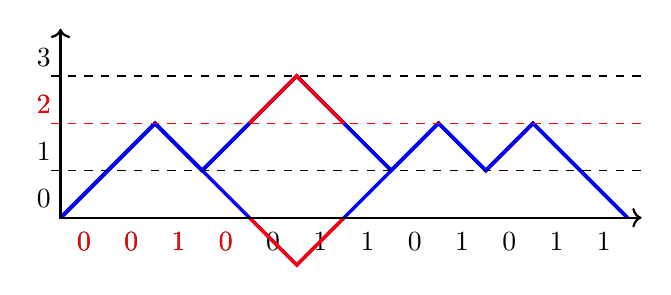
\begin{tikzpicture}[scale=.6]
    \visible<-2, 4-7>{
        \draw (.5, -.5) node {0};}
    \visible<-3, 5-7>{
        \draw (1.5, -.5) node {0};}
    \visible<-4, 6,7>{
        \draw (2.5, -.5) node {1};}
    \visible<-5,7>{
        \draw (3.5, -.5) node {0};}

    \visible<3>{
        \draw[red] (.5, -.5) node {0};}
    \visible<4>{
        \draw[red] (1.5, -.5) node {0};}
    \visible<5>{
        \draw[red] (2.5, -.5) node {1};}
    \visible<6>{
        \draw[red] (3.5, -.5) node {0};}

    \visible<-7> {
        \draw (4.5, -.5) node {0};
        \draw (5.5, -.5) node {1};
        \draw (6.5, -.5) node {1};
        \draw (7.5, -.5) node {0};
        \draw (8.5, -.5) node {1};
        \draw (9.5, -.5) node {0};
        \draw (10.5, -.5) node {1};
        \draw (11.5, -.5) node {1};}

    \visible<3>{
        \draw[red, very thick] (0, 0) -- (1, 1);
    }

    \visible<4>{
        \draw[blue, very thick] (0,0) -- (2, 2);
        \draw[red, very thick] (1, 1) -- (2, 2);
    }

    \visible<5>{
        \draw[blue, very thick] (0, 0) -- (2, 2) -- (3, 1);
        \draw[red, very thick] (2, 2) -- (3, 1);
    }

    \visible<6>{
        \draw[blue, very thick] (0, 0) -- (2, 2) -- (3, 1) -- (4, 2);
        \draw[red, very thick] (3, 1) -- (4, 2);
    }

    \visible<7>{
        \draw[blue, very thick] (0, 0) -- (2, 2) -- (3, 1) -- (5, 3) -- (7, 1) -- (8, 2) -- (9, 1) -- (10, 2) -- (12, 0);
    }

    \visible<8>{
        \draw[blue, very thick] (0, 0) -- (2, 2) -- (3, 1) -- (5, 3) -- (7, 1) -- (8, 2) -- (9, 1) -- (10, 2);
        \draw[very thick, red] (9,1) -- (10, 2);
    }
    \visible<9>{
        \draw[blue, very thick] (0, 0) -- (2, 2) -- (3, 1) -- (5, -1) -- (7, 1) -- (8, 2) -- (9, 1) -- (10, 2) -- (12, 0);
        \draw[very thick, red] (4, 0) -- (5, -1) -- (6, 0);
    }

    \visible<10>{
        \draw[blue, very thick] (0, 0) -- (2, 2) -- (3, 1) -- (5, 3) -- (7, 1) -- (8, 2) -- (9, 1) -- (10, 2) -- (12, 0);
    }


    \visible<2->{
        \draw[<->, thick] (0, 4) -- (0, 0)  -- (12.3, 0);
        \draw[dashed] (-.2, 1) -- (12.3, 1);
        \draw[dashed] (-.2, 3) -- (12.3, 3);
        \draw (0, 0) node[above left] {0};
        \draw (0, 1) node[above left] {1};
        \draw (0, 3) node[above left] {3};}
    \visible<2-9>{
        \draw (0, 2) node[above left] {2};
        \draw[dashed] (-.2, 2) -- (12.3, 2);}
    \visible<10>{
        \draw[red] (0, 2) node[above left] {2};
        \draw[red,dashed] (-.2, 2) -- (12.3, 2);
        \draw[very thick, red] (4, 2) -- (5, 3) -- (6, 2);
    }



\end{tikzpicture}
    \end{figure}
    \visible<9>{
        {\Huge \[\Dyck{k}\]}}
\end{frame}

\subsection{History and state of the art}

\begin{frame}
    \frametitle{A result which does not answer fully the $Q(\Dyck{k})$ problem.}
    \vfill
    \textbf{The Trichotomy theorem:}(Aaronson,
    Grier and Schaeffer \cite[2019]{trichotomy_not_andris})
    \begin{center}
        {\huge Star Free Languages $\implies \Theta\left(\sqrt{n}(\log_2(n))^c\right)$ }\\
    \end{center}
    \vfill
    \pause
    \textbf{Application:}
    \begin{center}
        {\huge \Dyck{k} $\in$ Star free languages}
    \end{center}
    \pause
    \vfill
    \textbf{Implication:}
    \begin{center}
        {\huge $\comment{\exists p, }Q(\Dyck{k})=\Theta \left(\sqrt{n}\log_2(n)^{p(k)}\right)$}
    \end{center}
    \vfill
\end{frame}

\begin{frame}
    \frametitle{First step, one try to have a good upper bounds.}

    \begin{itemize}
        \item \textbf{Algorithms:} A. Ambainis and al. \cite[2020]{art:2DGrid}
              {\huge \[Q(\Dyck{k}) = O\left(\sqrt{n}(\log_2(n))^{0.5k}\right)\]}
              \pause
        \item \textbf{Reductions to:}
              \begin{figure}
                  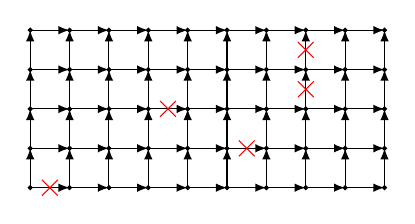
\begin{tikzpicture}[scale=.5]
                      \foreach \j in {0, ..., 3} {
                              \foreach \i in {0, ..., 9} {
                                      \draw[-latex] (\i, \j) -- (\i,\j+1);
                                  }}
                      \foreach \j in {0, ..., 4} {
                              \foreach \i in {0, ..., 9} {
                                      \draw[fill=black] (\i, \j) circle (.05);
                                  }}
                      \foreach \j in {0, ..., 4} {
                              \foreach \i in {0, ..., 8} {
                                      \draw[-latex] (\i, \j) -- (\i+1,\j);
                                  }}
                      \draw[red] (.3, .2) -- (.7, -.2);
                      \draw[red] (.3, -.2) -- (.7, .2);

                      \draw[red] (3+.3, .2+2) -- (3+.7, -.2+2);
                      \draw[red] (3+.3, -.2+2) -- (3+.7, .2+2);

                      \draw[red] (5+.3, .2+1) -- (5+.7, -.2+1);
                      \draw[red] (5+.3, -.2+1) -- (5+.7, .2+1);

                      \draw[red] (-.5+7+.3, .2+2+.5) -- (-.5+7+.7, -.2+2+.5);
                      \draw[red] (-.5+7+.3, -.2+2+.5) -- (-.5+7+.7, .2+2+.5);

                      \draw[red] (6.5+.3, .2+3.5) -- (6.5+.7, -.2+3.5);
                      \draw[red] (6.5+.3, -.2+3.5) -- (6.5+.7, .2+3.5);
                  \end{tikzpicture}
                  \caption{A reduction to 2D directed grid connectivity.}
              \end{figure}
              {\huge \[Q(\Dyck{k}) = O\left(\sqrt{n}(\log_2(n))^{0.5(k-1)}\right)\]}
    \end{itemize}

\end{frame}


\begin{frame}
    \frametitle{Second step, one try to prove the optimality with a matching lower bound.}
    \begin{itemize}
        \item \textbf{Adversary methods:}
              \begin{align*}
                  \textsc{Ex}_{2m}^{m|m+1}(x)=0 & \Leftrightarrow |x|_0-|x|_1 = 2 \\
                  \textsc{Ex}_{2m}^{m|m+1}(x)=1 & \Leftrightarrow |x|_0-|x|_1 = 0 \\
              \end{align*}
              {\huge \[Q(\textsc{Ex}_{2m}^{m|m+1}) = \Omega\left(m\right)\]}
              \pause
        \item \textbf{Reduction from:} $\textsc{Ex}_{2m}^{m|m+1} \leq \Dyck{k,n}$
              {\huge \[Q(\Dyck{k}) = \Omega\left(\sqrt{n}c^{k}\right)\]}
    \end{itemize}
\end{frame}

\begin{frame}
    \frametitle{A natural goal is to made the bounds match.}
    \begin{figure}
        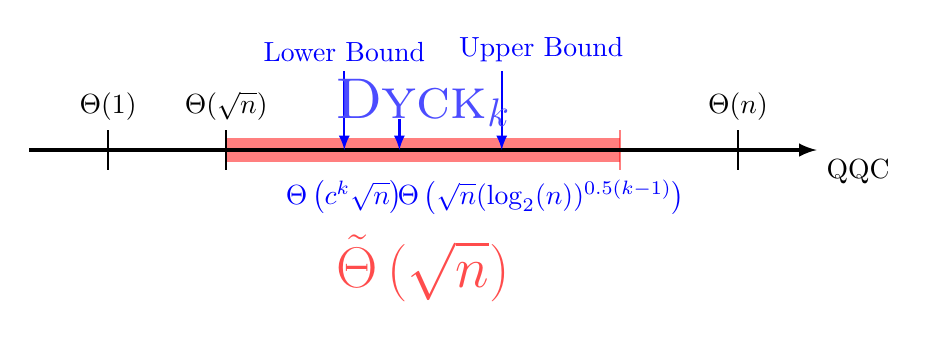
\begin{tikzpicture}
            \draw (10, 0) node[below right] {QQC};
            \draw[opacity=0, fill=red, fill opacity=.5 ] (2.5, .15) -- (2.5, -.15) -- (7.5, -.15) -- (7.5, .15) -- cycle;
            \draw[red, opacity=.5, thick] (7.5, .25) -- (7.5, -.25);
            \draw[red!70] (5, -1.5) node {\huge $\tilde{\Theta}\left(\sqrt{n}\right)$};
            \draw[-latex, very thick] (0, 0) -- (10, 0);
            \draw[thick] (1, .25) -- (1, -.25);
            \draw (1, .25) node[above] {$\Theta(1)$};
            \draw[thick] (9, .25) -- (9, -.25);
            \draw (9, .25) node[above] {$\Theta(n)$};
            \draw[thick] (2.5, .25) -- (2.5, -.25);
            \draw (2.5, .25) node[above] {$\Theta(\sqrt{n})$};
            \draw[blue, thick, -latex] (4, 1) -- (4, 0);
            \draw[blue] (4, -.6) node {$\Theta \left(c^k\sqrt{n}\right)$};
            \draw[blue] (4, 1) node[above] {Lower Bound};
            \draw[blue, thick, -latex] (6, 1) -- (6, 0);
            \draw[blue] (6.5, -.6) node {$\Theta \left(\sqrt{n}(\log_2(n))^{0.5(k-1)}\right)$};
            \draw[blue] (6.5, 1) node[above] {Upper Bound};

            %\draw[opacity=0, fill=blue, fill opacity=.5 ] (4, .15) -- (4, -.15) -- (6, -.15) -- (6, .15) -- cycle;
            \draw[blue!70] (5, .6) node {\huge \Dyck{k}};
            \draw[blue, thick, -latex] (4.7, .4) -- (4.7, 0);

        \end{tikzpicture}
        \caption{Representation of the different bounds.}
    \end{figure}
\end{frame}




\section[The progress to reduce QQC of bounded height Dyck word]{The progress to reduce Quantum Query Complexity of bounded height Dyck word}

\subsection{The problem is not only a grover search.}

\begin{frame}
    \frametitle{Every $k$ is not as simple as 1.}
    \begin{minipage}{.45\textwidth}
        \begin{itemize}
            \item \textbf{\huge $k=1$:}
        \end{itemize}
        \begin{figure}
            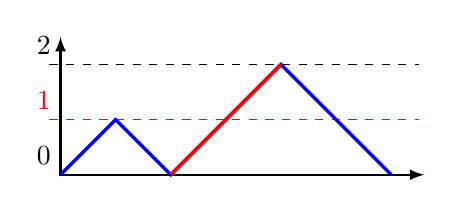
\begin{tikzpicture}[scale=.7]
                \visible<1->{
                    \draw[latex-latex, thick] (0, 2.5) -- (0, 0)  -- (6.6, 0);
                    \draw[red, dashed] (-.2, 1) -- (6.5, 1);
                    \draw[dashed] (-.2, 2) -- (6.5, 2);
                    \draw (0, 0) node[above left] {0};
                    \draw[red] (0, 1) node[above left] {1};
                    \draw (0, 2) node[above left] {2};
                    \draw[blue, very thick] (0, 0) -- (1, 1) -- (2, 0) -- (4, 2) -- (6, 0);}
                \visible<2->{
                    \draw[red, very thick] (2, 0) -- (4, 2);}
            \end{tikzpicture}
            \caption{A dyck word of height 2.}
        \end{figure}
        \visible<2->{
            {\huge \[O\left(\sqrt{n}\right)\]}}
    \end{minipage}
    \hfill
    \begin{minipage}{.45\textwidth}
        \visible<3->{
            \begin{itemize}
                \item \textbf{\huge $k=2$:}
            \end{itemize}}
        \begin{figure}
            \vspace*{-.2cm}
            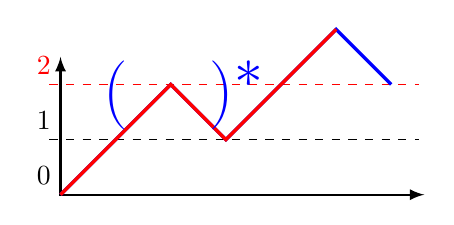
\begin{tikzpicture}[scale=.7]
                \visible<3->{
                    \draw[latex-latex, thick] (0, 2.5) -- (0, 0)  -- (6.6, 0);
                    \draw[dashed] (-.2, 1) -- (6.5, 1);
                    \draw[red, dashed] (-.2, 2) -- (6.5, 2);
                    \draw (0, 0) node[above left] {0};
                    \draw (0, 1) node[above left] {1};
                    \draw[red] (0, 2) node[above left] {2};
                    \draw[blue, very thick] (0, 0) -- (2, 2) -- (3, 1) -- (5, 3) -- (6, 2);}
                \visible<4->{
                    \draw[red, very thick] (0, 0) -- (2, 2) -- (3, 1) -- (5, 3);
                    \draw[blue] (1, 1) node[above] {\Huge $($};
                    \draw[blue] (3.2, 1) node[above] {\Huge $)^*$};}
            \end{tikzpicture}
            \visible<3->{\caption{A substring of height 3.}}
        \end{figure}
        \visible<5->{
            {\huge \[O\left(n\sqrt{n}\right)\]}}

    \end{minipage}


\end{frame}

\begin{frame}
    \frametitle{Small definitions and intuitions.}

    \begin{minipage}{.45\textwidth}
        \begin{itemize}
            \item \textbf{$\pm k$ strings: $\phantom{decomposition}$}
        \end{itemize}
        \begin{figure}
            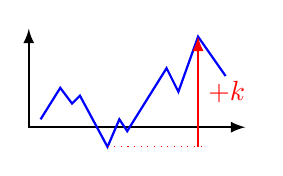
\begin{tikzpicture}[scale=.5]
                \draw[latex-latex, thick] (0, 2.5) --(0, 0) -- (5.5, 0);
                \draw[blue, thick] (0.3, 0.2) -- (.8, 1 ) -- (1.1, .6)
                -- (1.3, .8) -- (2, -.5) -- (2.3, .2) -- (2.5, -.1) --
                (3.5, 1.5) -- (3.8, 0.9) -- (4.3, 2.3) -- (5, 1.3);
                \draw[dotted, red] (2, -.5) -- (4.5, -.5);
                \draw[-latex, red, thick] (4.3, -.5) --node[right] {$+ k$} (4.3, 2.3);
            \end{tikzpicture}
            \caption{Representation of a $+k$-string.}
        \end{figure}
    \end{minipage}
    \pause
    \hfill
    \begin{minipage}{.45\textwidth}
        \begin{itemize}
            \item \textbf{Minimal decomposition:}
        \end{itemize}
        \vspace*{-.2cm}
        \begin{figure}
            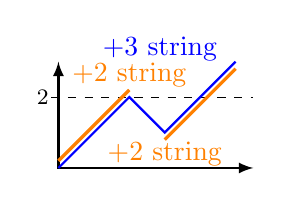
\begin{tikzpicture}[scale=.45]
                \draw[latex-latex, thick] (0, 3) -- (0, 0) -- (5.5, 0);
                \foreach \j in {2} {
                        \draw[dashed] (-.2, \j) -- (5.5, \j);
                        \draw (0, \j) node[left] {\footnotesize \j};
                    }
                \draw[blue, thick] (0, 0) -- (2, 2) -- (3, 1) -- (5, 3);
                \draw[blue] (4.75, 2.75) node[above left] {+3 string};

                \draw[orange, very thick] (0, 0+.2) -- (2, 2+.2);
                \draw[orange] (2,2) node[above] {+2 string};
                \draw[orange, very thick] (3, 1-.2) -- (5, 3-.2);
                \draw[orange] (3, 1) node[below] {+2 string};
            \end{tikzpicture}
            \caption{A +3 string decomposition.}
        \end{figure}
    \end{minipage}
\end{frame}

\subsection{Original algorithm and small updates }

\begin{frame}
    \frametitle{A. Ambainis and all. first inductive algorithm in  $\tilde{\Theta}\left(\sqrt{n}\right)$.}
    \begin{minipage}{.5\textwidth}
        \begin{figure}
            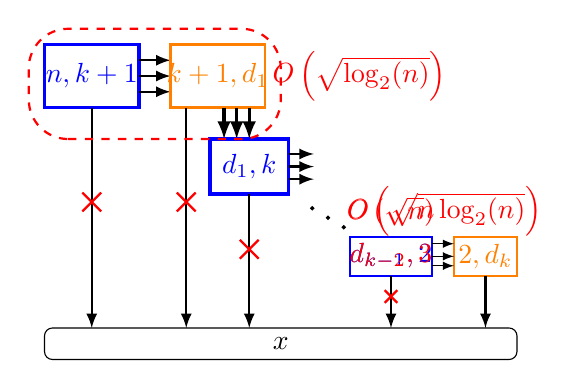
\begin{tikzpicture}[scale=.4]
                \visible<1->{
                    \draw[rounded corners=.1cm] (0, -7) -- (0, -8) -- (15, -8) -- (15, -7) -- cycle;
                    \draw (7.5, -7.5) node {$x$};
                }
                \visible<1->{
                    \draw[blue, very thick] (0, 0) -- (3, 0) -- (3, 2) -- (0, 2) -- cycle;
                    \draw[blue] (1.5, 1) node {$n,k+1$};
                    \draw[thick, -latex] (1.5, 0) -- (1.5, -7);
                    \draw[red, thick] (1.2, -2.7) -- (1.8, -3.3);
                    \draw[red, thick] (1.2, -3.3) -- (1.8, -2.7);
                }
                \visible<2->{
                    \draw[-latex, thick] (3, 1) -- (4, 1);
                    \draw[-latex, thick] (3, .5) -- (4, .5);
                    \draw[-latex, thick] (3, 1.5) -- (4, 1.5);
                    \draw[orange, thick] (4, 0) -- (4, 2) -- (7, 2) -- (7, 0) -- cycle;
                    \draw[orange] (5.5, 1) node {$k+1,d_1$};
                    \draw[thick, -latex] (4.5, 0) -- (4.5, -7);
                    \draw[red, thick] (4.2, -2.7) -- (4.8, -3.3);
                    \draw[red, thick] (4.2, -3.3) -- (4.8, -2.7);
                }
                \visible<3->{
                    \draw[-latex, very thick] (6.5, 0) -- (6.5, -1);
                    \draw[-latex, very thick] (6.1, 0) -- (6.1, -1);
                    \draw[-latex, very thick] (5.7, 0) -- (5.7, -1);
                    \draw[blue, very thick] (5.25, -1) -- (7.75, -1) -- (7.75, -2.75) -- (5.25, -2.75) -- cycle;
                    \draw[blue] (6.5, -1.875) node {$d_1,k$};
                }
                \visible<4->{
                    \draw[thick, -latex] (6.5, -2.75) -- (6.5, -7);
                    \draw[red, thick] (6.2, -2.7-1.5) -- (6.8, -3.3-1.5);
                    \draw[red, thick] (6.2, -3.3-1.5) -- (6.8, -2.7-1.5);
                    \draw[thick, -latex] (7.75, -1.875) -- (7.75+.8, -1.875);
                    \draw[thick, -latex] (7.75, -1.875-.4) -- (7.75+.8, -1.875-.4);
                    \draw[thick, -latex] (7.75, -1.875+.4) -- (7.75+.8, -1.875+.4);
                    \draw[fill=black] (8.5, -3.2) circle (.05);
                    \draw[fill=black] (9, -3.5) circle (.05);
                    \draw[fill=black] (9.5, -3.8) circle (.05);
                    \draw[blue, thick] (9.7, -4.1) -- (12.3, -4.1) -- (12.3, -5.35) -- (9.7, -5.35)--cycle;

                    \draw[-latex, thick] (11, -5.35) -- (11, -7);
                }
                \visible<4-5>{
                    \draw[orange, thick] (13, -4.1) -- (15, -4.1) -- (15, -5.35) -- (13, -5.35) -- cycle;
                    \draw[orange] (14, -4.725) node {$2,d_k$};
                    \draw[-latex] (12.3, -4.725) -- (13, -4.725);
                    \draw[-latex] (12.3, -4.325) -- (13, -4.325);
                    \draw[-latex] (12.3, -5.025) -- (13, -5.025);
                    \draw[-latex, thick] (14, -5.35) -- (14, -7);
                    \draw[red, thick] (10.8, -5.8) -- (11.2, -6.2);
                    \draw[red, thick] (10.8, -6.2) -- (11.2, -5.8);}

                \visible<4-7>{
                    \draw[blue] (11, -4.725) node {$d_{k-1}, 2$};}
                \visible<8>{\draw[red] (11, -4.725) node {$d_{k-2}, 3$};}

                \visible<5->{
                    \draw[red, thick, dashed, rounded corners=.5cm] (-.5, -1) -- (7.5, -1) -- (7.5, 2.5) -- (-.5, 2.5) -- cycle;
                    \draw[red] (10, 1) node {$O\left(\sqrt{\log_2(n)}\right)$};}
                \visible<5>{
                    \draw[red] (12.7, -3.3) node {$O\left(\sqrt{n\log_ 2(n)}\right)$};
                }
                \visible<6->{\draw[red] (11, -3.3) node {$O\left(\sqrt{n}\right)$};}
            \end{tikzpicture}
            \caption{Schema to present the idea of the original algorithm. Not show the real
                computation of the QQC.}
        \end{figure}
    \end{minipage}
    \hfill
    \begin{minipage}{.4\textwidth}
        \begin{itemize}
            \visible<5->{
            \item \textbf{Original QQC:}
                  \[O\left(\sqrt{n}(\log_2(n))^{0.5k}\right)\]}
                  \visible<6->{
            \item \textbf{Small update:}
                  \[O\left(\sqrt{n}(\log_2(n))^{0.5(k-1)}\right)\]}
                  \visible<7->{
            \item \textbf{Bigger update:}
                  \[O\left(\sqrt{n}(\log_2(n))^{0.5(k-2)}\right)\]}
        \end{itemize}
    \end{minipage}
\end{frame}

\subsection{A new algorithm for k=2}

\begin{frame}
    \frametitle{An easy and fast algorithm exists for k=2.}

    \begin{minipage}{.45\textwidth}
        \begin{itemize}
            \item \textbf{Highest +2-substring:}
        \end{itemize}
        \begin{figure}
            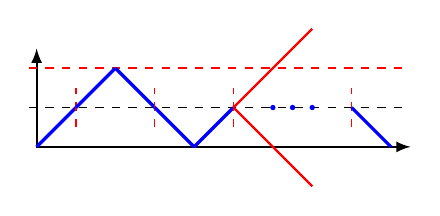
\begin{tikzpicture}[scale=.5]
                \visible<1->{
                    \draw[latex-latex, thick] (0, 2.5) -- (0, 0) -- (9.5, 0);
                    \draw[red, dashed, thick] (-.2, 2) -- (9.5, 2);
                    \draw[dashed] (-.2, 1) -- (9.5, 1);
                    \draw[blue, very thick] (0, 0) -- (1,1);
                    \draw[red, dashed] (1, .5) -- (1, 1.5);
                }
                \visible<2->{
                    \draw[blue, very thick] (1,1) -- (2, 2);
                    \draw[blue, very thick] (2, 2) -- (3, 1);
                    \draw[dashed, red] (3, .5) -- (3, 1.5);
                }
                \visible<3->{
                    \draw[blue, very thick] (3,1) -- (4, 0);
                    \draw[blue, very thick] (4, 0) -- (5, 1);
                    \draw[dashed, red] (5, .5) -- (5, 1.5);
                }
                \visible<4->{
                    \draw[blue ,fill=blue] (6, 1) circle (1.5pt);
                    \draw[blue, fill=blue] (6.5, 1) circle (1.5pt);
                    \draw[blue, fill=blue] (7, 1) circle (1.5pt);
                    \draw[dashed, red] (8, .5) -- (8, 1.5);
                    \draw[blue, very thick] (8, 1) -- (9, 0);
                }
                \visible<5>{
                    \draw[red, thick] (5, 1) -- (7, -1);
                }

                \visible<6->{
                    \draw[red, thick] (5, 1) -- (7, 3);
                }
            \end{tikzpicture}
        \end{figure}
    \end{minipage}
    \hfill
    \begin{minipage}{.45\textwidth}
        \visible<7->{
            \begin{itemize}
                \item \textbf{Lowest +2-substring:}
            \end{itemize}}
        \begin{figure}
            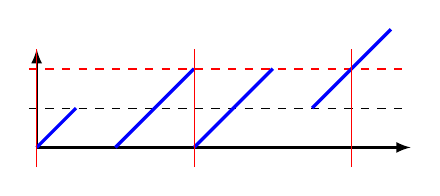
\begin{tikzpicture}[scale=.5]
                \visible<7->{
                    \draw[latex-latex, thick] (0, 2.5) -- (0, 0) -- (9.5, 0);
                    \draw[red, dashed, thick] (-.2, 2) -- (9.5, 2);
                    \draw[dashed] (-.2, 1) -- (9.5, 1);
                    \draw[blue, very thick] (0, 0) -- (1,1);
                    \draw[blue, very thick] (7, 1) -- (9, 3);

                    \draw[blue, very thick] (2, 0) -- (4, 2);
                    \draw[blue, very thick] (4, 0) -- (6, 2);

                    \draw[red] (0, -.5) -- (0, 2.5);
                    \draw[red] (8, -.5) -- (8, 2.5);
                    \draw[red] (4, -.5) -- (4, 2.5);}

            \end{tikzpicture}
        \end{figure}
    \end{minipage}
    {\large \[\visible<8->{Q(\Dyck{2,n}) = O\left(\sqrt{n}\right)} \visible<9->{\implies Q(\Dyck{k,n})= O\left(\sqrt{n}(\log_2(n))^{0.5(k-2)}\right)}\]}
\end{frame}

\section{New idea to get better quantum query complexity bounds }

\subsection{For lower bounds}
\begin{frame}
    \frametitle{A better reduction can increse the lower bounds.}
    \begin{itemize}
        \item Tightness of $\textsc{Ex}_{2m}^{m|m+1}$'s one.
        \item New problem for a new reduction:
              \[\textsc{Ex}_{2m}^{m|m+1} \leq\ new\ problem\ \leq \Dyck{k}.\]
    \end{itemize}
\end{frame}

\subsection{For upper bounds:}
\begin{frame}
    \frametitle{Optimizing the recursion step of Ambainis and all. algorithm can decrease the upper bound.}
    \begin{minipage}{.45\textwidth}
        \begin{figure}
            \begin{algorithmic}
                \For{$1 \leq d_1 \leq \log_2(n)$}
                \For{$1 \leq d_2 < d_1$}
                \State $\ddots$
                \For{$1\leq d_{k-1} < d_{k-2}$}
                \State \texttt{Find a} $\pm(k+1)$-string
                \EndFor
                \EndFor
                \EndFor
            \end{algorithmic}
            \caption{Inexact simplification of the original algorithm.}
        \end{figure}
    \end{minipage}
    \hfill
    \begin{minipage}{.45\textwidth}
        \begin{figure}
            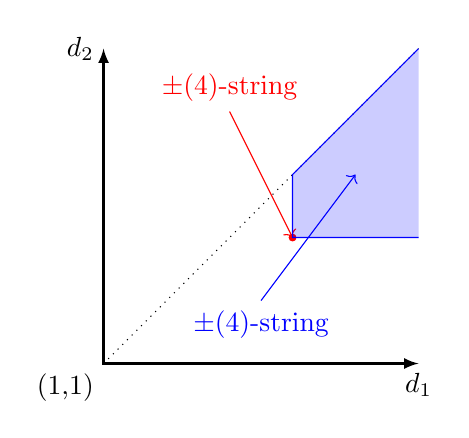
\begin{tikzpicture}[scale=.4]
                \visible<2->{
                    \draw[thick, latex-latex] (0, 10) -- (0, 0) -- (10, 0);
                    \draw (10, 0) node[below] {$d_1$};
                    \draw (0, 10) node[left] {$d_2$};
                    \draw[dotted] (0, 0) -- (10, 10);
                    \draw (0, 0) node[below left] {(1,1)};}
                \visible<3->{
                    \draw[red, fill = red] (6, 4) circle (3pt);
                    \draw[red, <- ] (6, 4) -- (4, 8) node[above] {$\pm(4)$-string};
                }
                \visible<4->{
                    \draw[fill = blue, fill opacity=.2, blue] (10, 10) -- (6, 6) -- (6, 4) -- (10, 4);
                    \draw[blue, <- ] (8, 6) -- (5, 2) node[below] {$\pm(4)$-string};}
            \end{tikzpicture}
            \visible<2->{
                \caption{Graph for $k=4$.}}
        \end{figure}
    \end{minipage}
\end{frame}
\subsection{Conclusion}

\begin{frame}
    \frametitle{To conclude:}
    \textbf{What has been done:}
    \begin{itemize}
        \item Trichotomy
        \item Adversary methods
        \item Reduction methods
        \item New algorithm: $O\left(\sqrt{n}(\log_2(n))^{0.5k}\right) \rightarrow O\left(\sqrt{n}(\log_2(n))^{0.5(k-2)} \right)$
    \end{itemize}
    \pause
    \textbf{Possible idea to go further:}
    \begin{itemize}
        \item Prove that new upper bound approach cannot work
        \item New algorithm
        \item General Adversary method
    \end{itemize}

\end{frame}


\begin{frame}
    \centering
    {\Huge
        Thanks for your attention.\\[1cm]

        Question Time\\[1cm]}


    \bibliographystyle{plain}
    \bibliography{biblio}

\end{frame}

\end{document}
